\documentclass[a4paper]{article}
\usepackage{Graphicx}
\usepackage{fullpage}

\title{{RELACS: Reliable Estimator of Local Antagonizing and Counterproductive Sounds}}
\author{Steven Bosch \and Luuk Boulogne \and Pim van der Meulen \and Xeryus Stokkel  \and Rogier de Weert}

\begin{document}

\maketitle

\section{Product purpose}

\subsection{Problem}
Stress, the biggest problem of our society nowadays. Stress is very harmful to the health of a being, may it be a mouse or a man.
Stress causes problems in mental and in physical health, leading to many problems, one of which is a reduction in the urge to reproduce, another being less productive at work. 
Throughout the years, many methods have been devised to decrease stress and increase relaxation. 
The system described onward does not decrease stress or increases relaxation directly, but rather attends the user to the influence of stress-inducing sounds in the environment of the user.
When the user is more aware of stressful sounds its sound environment (also called soundscape) he or she could change this environment and might decrease their stress-level.

\subsection{Target group}
Stress is found in all living beings, young and old. But to narrow it down we devised a website that is only usable by human beings. 
(So NO robots.)
We could say that our target audience are students, people working in an office, construction workers, or the elderly, but this is clearly not the case. 
We like to think big and think of the complete (English-speaking) world as our target group, since everyone is influenced by stress. 
We think having a large target audience greatly improves the chances of success of a product. 
Anyone can benefit from our product, as everyone should be more aware of its surroundings and the effect of sound on a persons stress-level. 

\subsection{World improvement}
We aim to improve the world by making everyone more aware of their surroundings and the effects of sounds on their stress-level. 
By showing users that some of the sounds present in their environment are stress-inducing we want to improve the awareness of the importance of sound for a relaxed environment. 
We think that a relaxed environment would benefit a person, as productivity is higher when stress is lower.

\section{Product description}
In the next chapter the complete technical specifications can be found, followed by a performance analysis and a user manual. 
But first a simple representation of the working of RELACS is given. RELACS is a simple tool to see how stressful a sound-sample is. 
When a processed recording of 30 seconds is presented to the tool, it calculates the overall percentage of stressfulness of the sample and shows where in the sample the stressful sounds are located. 
Basically what RELACS does is: sound in, stress analysis out.

A processed recording means that a recording (.wav-file) should first be processed to a cochleogram (as in a .hdf5 file) before it can be presented to RELACS. The system then cuts the sample in windows of each 128

\section{Technical specifications}


\section{Performance analysis}

\subsection{Strengths}
\subsection{Weaknesses}
\subsection{Opportunities}
\subsection{Threats}


\section{User manual}
Currently RELACS only works web-based and with .hdf5 files as input. At the homepage a list of previous analyses can be found, with their respective stressful-percentage. This can be used to compare samples taken at a specific place, bt at a different time. The names of each 



\section{Pitch sheets}

\begin{figure*}[h]
\centering

\includegraphics[width=\linewidth]{./Slide1}
\label{fig:Slide1}
\end{figure*}

\begin{figure*}[h]
\centering
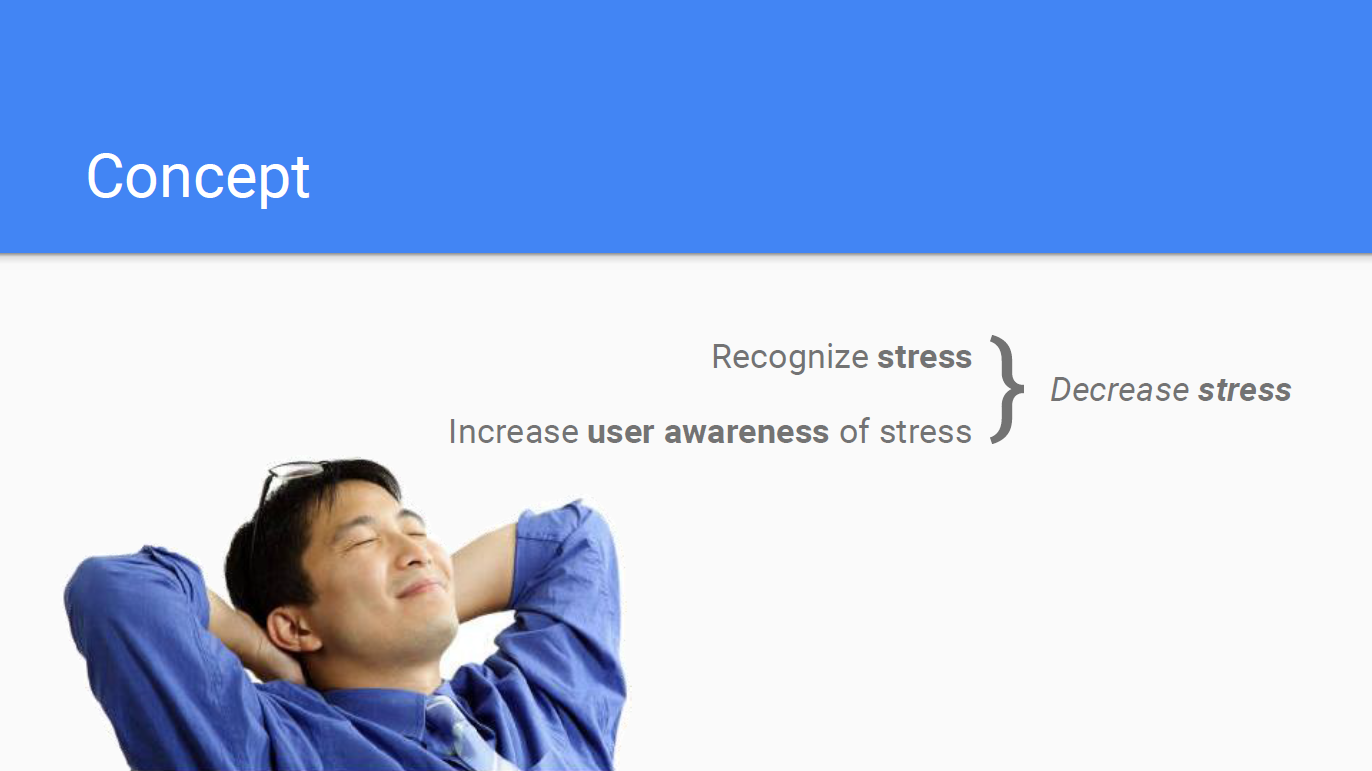
\includegraphics[width=\linewidth]{./Slide2}
\label{fig:Slide2}
\end{figure*}

\begin{figure*}[h]
\centering
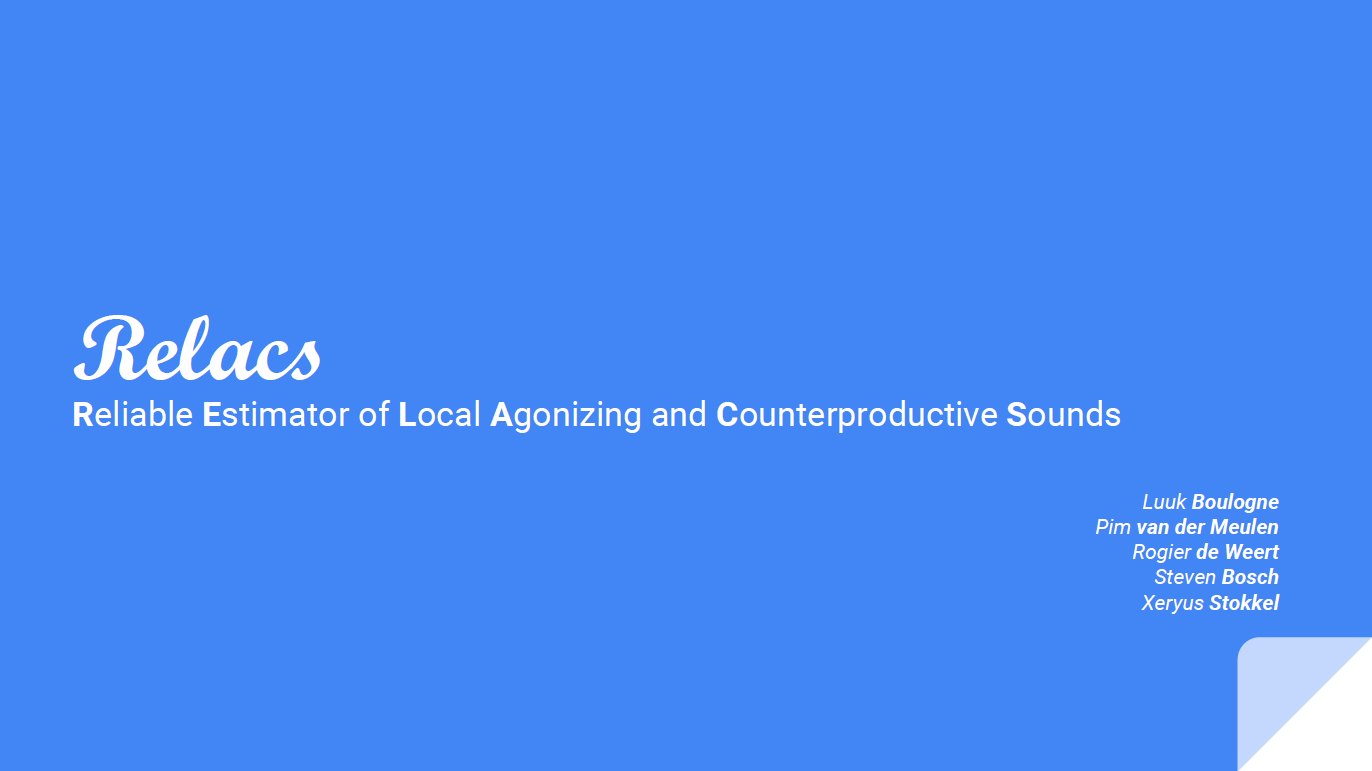
\includegraphics[width=\linewidth]{./Slide3}
\label{fig:Slide3}
\end{figure*}

\begin{figure*}[h]
\centering
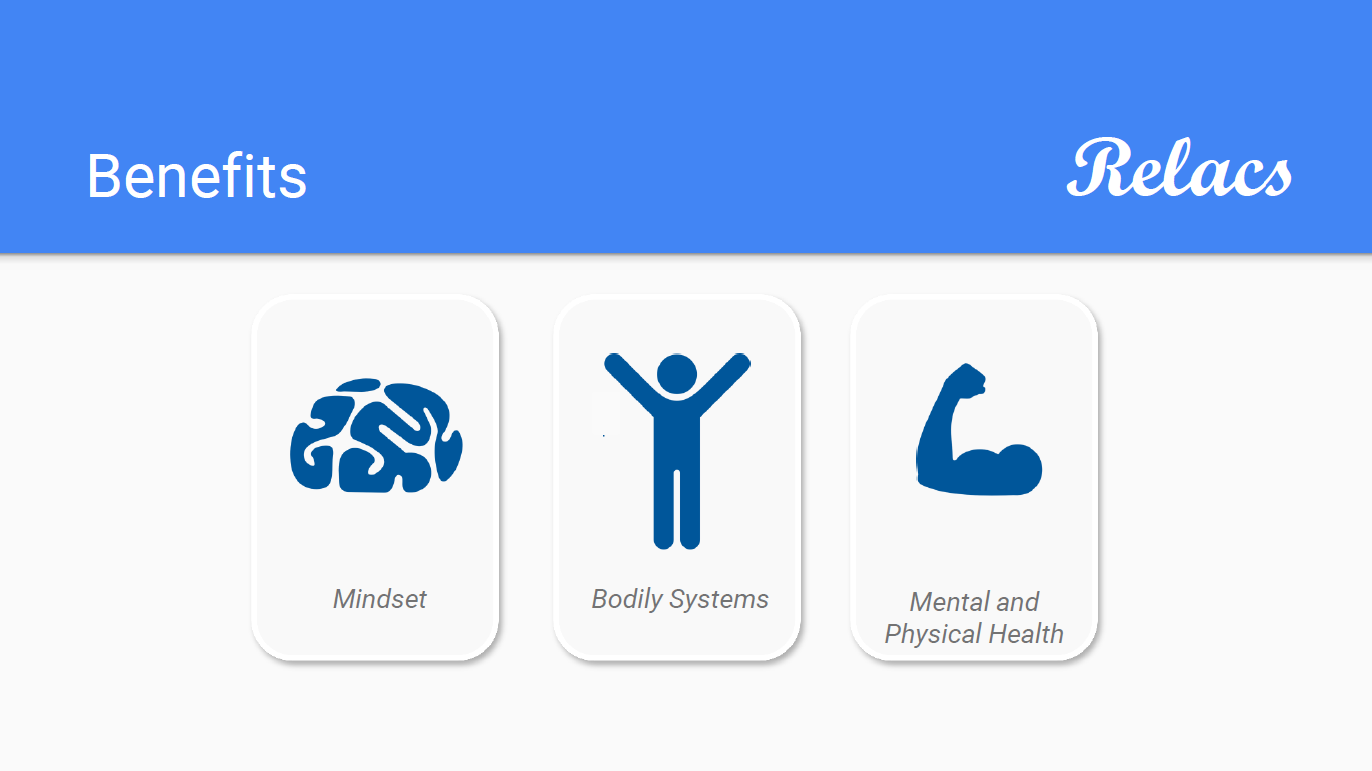
\includegraphics[width=\linewidth]{./Slide4}
\label{fig:Slide4}
\end{figure*}

\begin{figure*}[h]
\centering
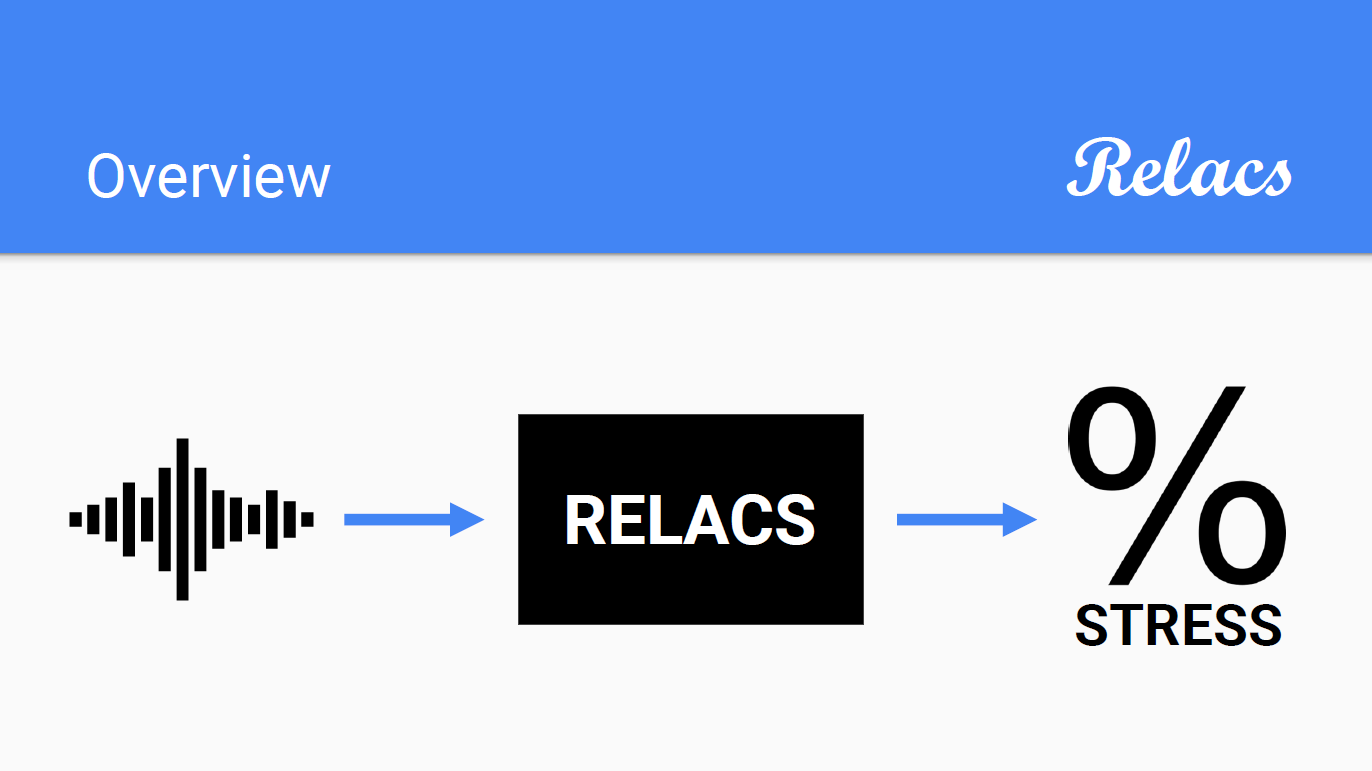
\includegraphics[width=\linewidth]{./Slide5}
\label{fig:Slide5}
\end{figure*}

\begin{figure*}[h]
\centering
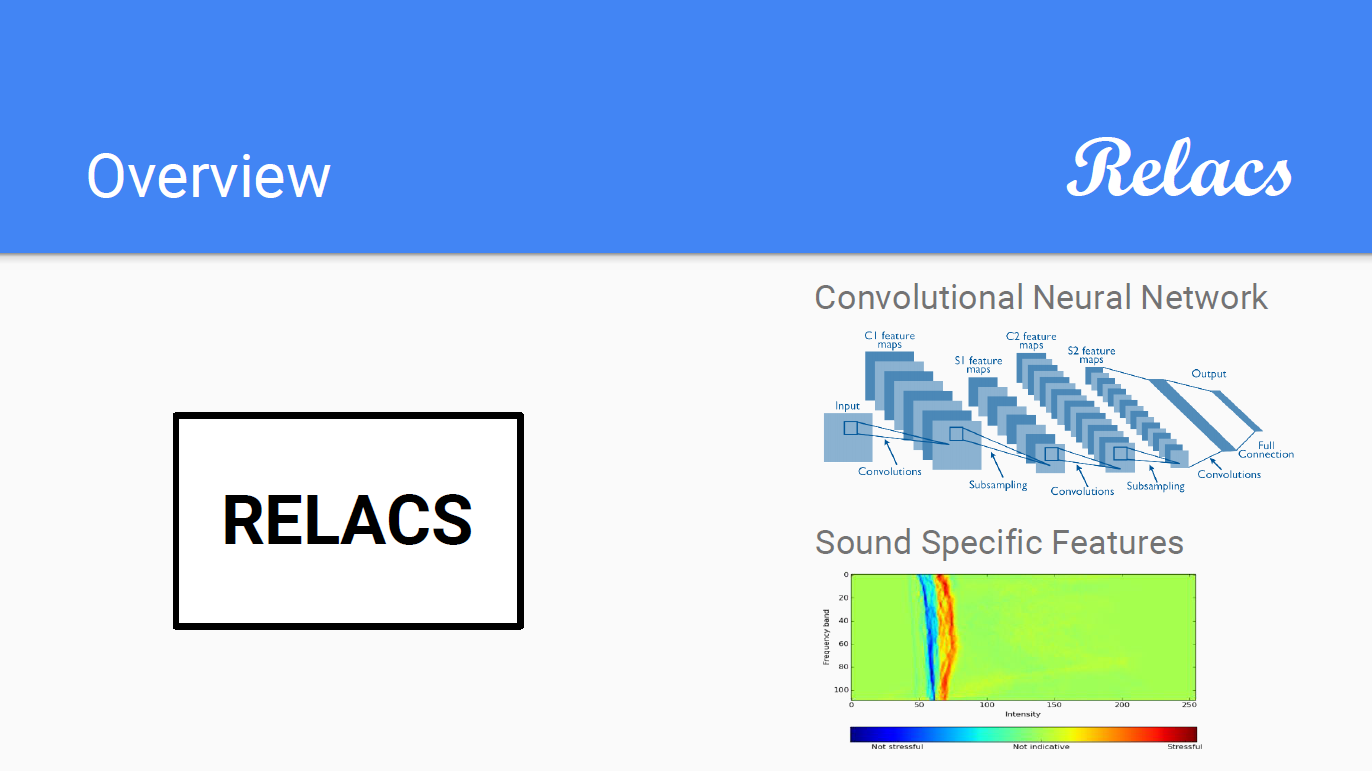
\includegraphics[width=\linewidth]{./Slide6}
\label{fig:Slide6}
\end{figure*}

\begin{figure*}[h]
\centering
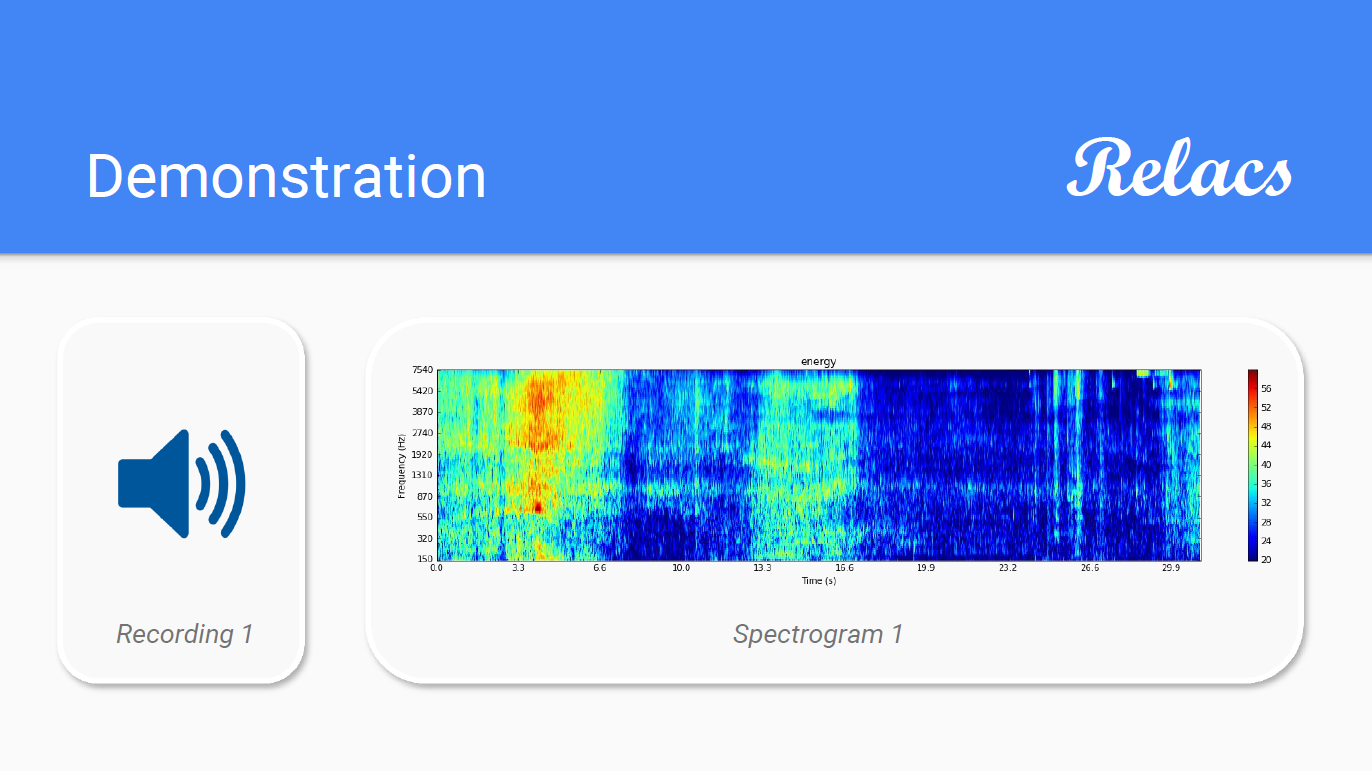
\includegraphics[width=\linewidth]{./Slide7}
\label{fig:Slide7}
\end{figure*}

\begin{figure*}[h]
\centering
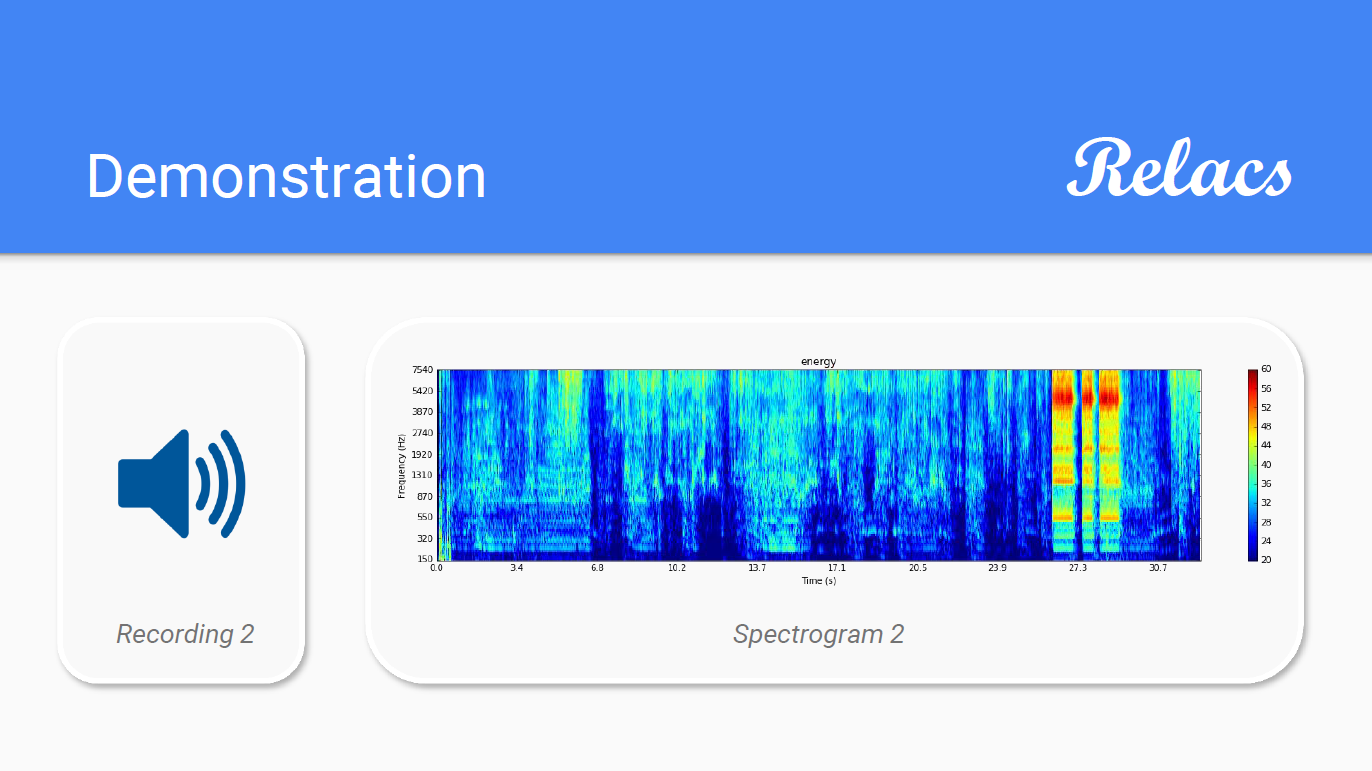
\includegraphics[width=\linewidth]{./Slide8}
\label{fig:Slide8}
\end{figure*}

\begin{figure*}[h]
\centering
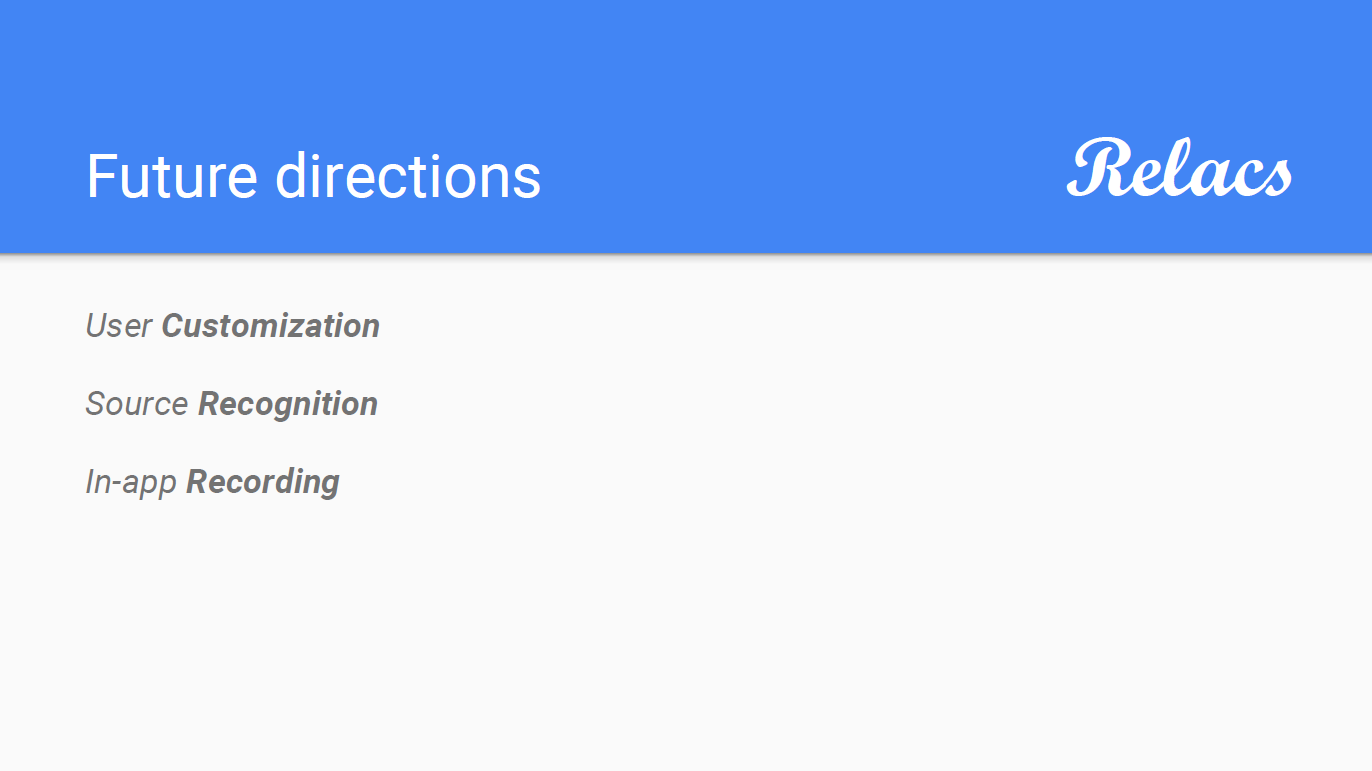
\includegraphics[width=\linewidth]{./Slide9}
\label{fig:Slide9}
\end{figure*}

\end{document}
